\documentclass[9pt,twocolumn,twoside,lineno]{pnas-new}
% Use the lineno option to display guide line numbers if required.
% https://www.pnas.org/authors/submitting-your-manuscript
\templatetype{pnasresearcharticle} % Choose template 
% {pnasresearcharticle} = Template for a two-column research article
% {pnasmathematics} %= Template for a one-column mathematics article
% {pnasinvited} %= Template for a PNAS invitedx submission

\title{Local similarity and global variability characterize the semantic space of human languages}

% Use letters for affiliations, numbers to show equal authorship (if applicable) and to indicate the corresponding author
\author[a,1]{Molly Lewis}
\author[b]{Aoife Cahill} 
\author[b]{Nitin Madnani}
\author[c,d,1]{James Evans}

\affil[a]{Carnegie Mellon University}
\affil[b]{Educational Testing Service}
\affil[c]{University of Chicago}
\affil[d]{Santa Fe Institute}

% Please give the surname of the lead author for the running footer
\leadauthor{Lewis} 

\significancestatement{The degree to which meanings align across the world’s languages suggests the limits of translation and cross-cultural communication. Approaching this question demands a systems-level view to compare the structure of meanings across many languages. Using machine learning we construct word embeddings -- dense, continuous, high-dimensional spaces that characterize word meanings from context -- across large samples of multi-lingual text. With these representations, we discover that (1) meanings across languages are similar within semantic domains and variable across them, and that (2) concrete meanings are less variable across languages than abstract ones, but all vary with distance. This suggests that associations and analogies, which interlink meanings within language, propose predictably different intuitions across distinct languages and confound the transmission of complex ideas.}

% Please include corresponding author, author contribution and author declaration information
\authorcontributions{JE and ML designed the research; ML analyzed all data; AC and NM ran the TOEFL models. JE and ML wrote the manuscript.}
%\authordeclaration{Please declare any competing interests here.}

\correspondingauthor{\textsuperscript{1}To whom correspondence should be addressed. E-mail:  jevans@uchicago.edu}

% At least three keywords are required at submission. Please provide three to five keywords, separated by the pipe symbol
\keywords{human cognition $|$ language $|$ semantics $|$ culture $|$ communication} 

\begin{abstract}
How does meaning vary across the world’s languages? Scholars recognize the existence of substantial variability within specific domains, ranging from nature and color to kinship. The emergence of large language models enables a systems-level approach that directly characterizes this variability through comparison of word organization across semantic domains. Here we show that meanings across languages manifest lower variability within semantic domains and greater variability between them, using models trained on both (1) large corpora of native language text comprising Wikipedia articles in 35 languages and also (2) English TOEFL essays written by 38,500 speakers from the same native languages, which cluster into semantic domains. Concrete meanings vary less across languages than abstract meanings, but all vary with geographical, environmental and cultural distance. By simultaneously examining local similarity and global difference, we harmonize these findings and provide the first description of general principles that govern variability in semantic space across languages. In this way, the structure of a speaker’s semantic space influences the comparisons cognitively salient to them, as shaped by their native language, and suggests that even successful bilingual communicators likely think with `semantic accents' driven by associations from their native language while writing English. These findings have dramatic implications for language education, cross-cultural communication, and literal translations, which are impossible not because the objects of reference are uncertain, but because associations, metaphors, and narratives interlink meanings in different, predictable ways from one language to another.
\end{abstract}

\dates{This manuscript was compiled on \today}
\doi{\url{www.pnas.org/cgi/doi/10.1073/pnas.XXXXXXXXXX}}

\begin{document}

\maketitle
\thispagestyle{firststyle}
\ifthenelse{\boolean{shortarticle}}{\ifthenelse{\boolean{singlecolumn}}{\abscontentformatted}{\abscontent}}{}

% If your first paragraph (i.e. with the \dropcap) contains a list environment (quote, quotation, theorem, definition, enumerate, itemize...), the line after the list may have some extra indentation. If this is the case, add \parshape=0 to the end of the list environment.
\dropcap{T}he degree to which word meanings vary across the world's languages and cultures is a fundamental question in the social and communication sciences. What precisely is the relationship between the meaning of words ``animal'', ``food'' and ``religion'' in English and their closest translations in Persian, Hindi and Russian? Variability in semantic structure is necessarily constrained by speakers' shared cognitive systems and the communicative functions demanded by social life
\cite{kay2006language,zaslavsky2019color,Regier2009language,wnuk2022color,majid2007semantic,jackson2019emotion,xu2020conceptual, gentner2009some, kemp2012kinship, majid2015can, regier2007color, Malt2003-vv}. Nevertheless, there is now evidence for substantial variability across languages regarding their semantic organization \cite{Bowerman2003-vn, Levinson2006-bs, Malt2003-cb, Regier2008-ut, gennari2002motion, choi1999early, majid2018differential, majid2014odors, huisman2021patterns,regier2016languages, kemmerer2019concepts, malt1999knowing}. %On the other hand, there is evidence that in cases of shared, concrete experiences, there is a high degree of semantic similarity across languages \cite{youn2016universal, wierzbicka1996semantics}. 
This evidence is primarily limited to the study of specific semantic domains, however, such as color \cite{berlin1991basic},  kinship \cite{murdock1970kin, kemp2012kinship}, and emotion \cite{jackson2019emotion}. 

In this paper, we describe and explore semantic variability by examining semantic relationships for many distinct languages \textit{across} referential domains, rather than within a single domain. By taking this ``system-level'' approach \cite{saussure, levi2008structural}, we seek to generalize prior work on meaning alignment to the macro {\it structure} of variability within and between semantic domains. Our results demonstrate variation within domains, with more concrete concepts translating more faithfully across languages than abstract ones. Moreover, we find substantially greater variation in meanings across domains. Languages manifest broad similarity in how they cluster words with meanings proximate to one another but diverge in how those clusters relate across semantic space. Across languages, meanings locally cohere but globally vary. For example, words associated with foods, body parts, spiritual agents, and human tragedies individually tend to cluster in similar ways, but relations between those clusters range widely by language.



Understanding the precise nature and degree of cross-linguistic semantic variability is important because it holds cognitive implications for our ability to learn and switch between languages, just as it pinpoints the pitfalls and potential of intercultural communication around the world \cite{marti2023latent}. To the extent that languages vary in their underlying meaning systems, the process of learning a language or translating an idea requires not only learning new word forms but also acquiring a rich representation of that system \cite{Lupyan_undated-du}. For example, when domains are close in a language's semantic space, the associations, analogies, metaphors, and narrative turns that interlink them may seem intuitive and common. By contrast, their linkage may seem strange and rare when domains are distant in semantic space. In this way, measured misalignment between close and distant concepts across language pairs would allow us to better characterize and predict the existence of ``semantic accents'' previously identified in bilingual speakers \cite{matsuki2021understanding, dong2005shared}, but on large scales across the world's languages. 

Examining lexical semantics at the system level presents several methodological challenges. Classic work on cross-linguistic semantics has explored the relationship between words within a single \cite[e.g.,][]{berlin1991basic,regier2007color,baddeley2009} or a few \cite{thompson2020cultural,xu2020conceptual, majid2015semantic} semantic domains. Researchers have pursued this approach in part because it is unclear how to compare diverse meanings: Red and pink can be compared along dimensions of lightness or saturation, but how does one compare the meaning of red to the meaning of mother? And yet, the relative position of diverse meanings condition the space of cognitively available associations. The domain-centric approach is further limited by its requirement that the analyst define relevant semantic domains of inquiry, thereby imposing idiosyncratic structure and the potential for bias.

Here we address these challenges by taking advantage of a recent advance in machine learning: neural network approaches to word embeddings \cite{bojanowski2016enriching,mikolov2013efficient}. Word embeddings provide a system-level description of semantics derived from the complex distribution of word collocations in a corpus of text. In the word embedding framework, each word is represented as a high dimensional (e.g., 200) vector, and distance between vectors corresponds to similarity between words, with closer words indicating more similar meanings. Word embeddings are highly correlated with human judgments of semantic similarity and encapsulate and represent culture-specific biases with fidelity \cite{hill2015simlex,caliskan2017semantics,garg2018word,bolukbasi2016man,kozlowski2019geometry,lewis2020, pereira2016comparative}. We describe computed word embeddings as representing the semantic space of a language and explore the semantic distance between pairs of languages in this space by evaluating continuous distances between word pairs in both. We then operationalize semantic domains by clustering words based on their loadings on embedding dimensions to compare ``local'' (within cluster) versus ``global'' (across cluster) variability in semantics between languages. We note that our distinction between `local' and `global' refers only to semantic distances within languages, synonymous with meanings that cluster versus those that span the language, and has no relationship with geographical distance. A positive correlation in word distances between two languages suggests that the two languages manifest similar relationships between lexical meanings, which we take as evidence for semantic similarity between those languages.

%expand on these in our methods section.

Using word embeddings, we compare the structure of semantic space for 35 different languages that span 11 language families in two stages and with two complementary datasets. First, we examine the direct relationship between concrete and abstract words, and between local and global word distances in the context of a large, naturalistic corpus of native language text, an embedding of all Wikipedia entries produced within each language. In Supplementary Figure S1, we show that for the 35 languages we examine, engagement with Wikipedia is comparable in terms of article production and consumption.

Second, we seek to validate these patterns, controlling for differences in topic, lexicon, and syntax, by analyzing TOEFL essays written in English by second-language learners from the corresponding languages. This allows us to examine the semantics of different languages without assuming translation equivalents of word meanings, and while holding constant native language grammar and lexicon. It also allows us to control for broad topic, as all essays are written in response to the same prompts (Fig.\ S2). The striking similarity of patterns between findings from these two datasets confirms that the semantics of one's native language influences the semantics of one's second language for bilingual speakers \cite{ameel2009semantic, malt2015bidirectional,ameel2005bilinguals, matsuki2021understanding, jarvis2008crosslinguistic, pavlenko2002bidirectional}, such that language learners from Athens ``think Greek'' while writing English. 

Together these two datasets provide converging evidence about the structure of meaning across human languages. We find substantial variability across languages in the structure of semantic space, but the relationship between the semantic systems of different languages is principled. Languages spoken by speakers culturally and geographically more similar manifest comparably similar semantic spaces. Furthermore, we find that the {\it ways} in which languages differ from each other is principled: Languages tend to vary much more across semantic domains than within them. 


%1. Validating the data: ETS & Wikipedia capturing the same cross language variation (1+)

%We trained word embedding models on text written by native speakers of 35 different languages, across 11 different language families, and compared these models to models trained on native language text. Essays written by speakers of the same language were much closer to essays written by speakers of the same native language, suggesting that models trained on second-language text were capturing native language semantics.

%\section*{Semantic difference between languages}
%\paragraph*

% Fig 1
\begin{figure*}[t!]
\centering
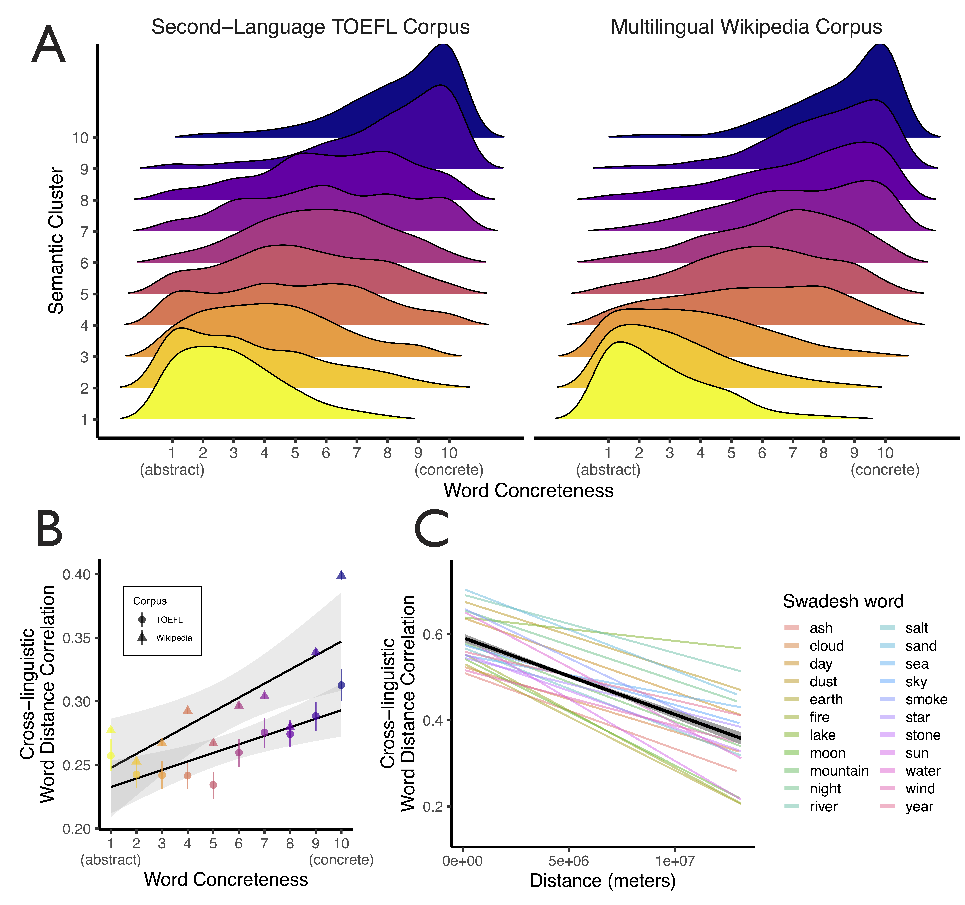
\includegraphics[width=15cm]{figs/fig1.pdf}
\caption{{\textbf A.} Distribution of words in each semantic cluster across concreteness deciles based on word embeddings obtained from Second-Language TOEFL Corpus and  Multilingual Wikipedia Corpus. {\textbf B.} Mean cross-linguistic word distance correlation (Pearson's $r$) as a function of the concreteness decile of the words. Larger values indicate more semantic similarity across languages. Point shape indicates corpus.  Point ranges correspond to bootstrapped 95\% confidence intervals; Range on model fit corresponds to the standard error. {\textbf C.} Linear model fits for cross-linguistic word distance correlation (Pearson's $r$) as a function of the geodesic distance between two languages (meters). Each data point corresponds to a unique language-pair-word combination. Colored lines correspond to the model fit for each word, and the black line shows the overall model fit and corresponding standard error.}
\label{fig:fig1} 
\end{figure*}




%2. Concrete similarity - Universalists
\section*{Concrete concepts translate better than abstract ones}
Having validated second-language text as a method for analyzing cross-linguistic semantic variability, we next examined cross-linguistic similarity in the structure of semantic space. We hypothesized that the {\it amount} of variability for a particular semantic domain across languages would vary, but in a principled manner. Following Gentner and colleagues \cite{Gentner1981-gs, Gentner1982-ro, Gentner_undated-wd, Zhou2021-dt}, we posit that semantic domains referring to meanings more \textit{perceptually} available and concrete such as ``food'' and ``body'' will be more similar across languages, relative to domains more conceptual and abstract like ``injustice'' and ``democracy''. This hypothesis has been motivated by the idea that, while there is substantial variability in the cultures and environments in which languages are spoken, all speakers share roughly the same perceptual systems and would therefore be more likely to experience similar concrete objects in similar ways \cite{rosch1975family, casasanto2011different}. 

To test the concreteness hypothesis, we estimated the concreteness of each word based on human judgments and partitioned them into 10 contiguous sets separated by rising concreteness thresholds  \cite{brysbaert2014concreteness} (Fig. S5). These sets overlapped strongly and significantly with semantic clusters in both the TOEFL ($\chi^2$(81) = 1538.1; $p$ $<$ .00001) and Wikipedia word samples ($\chi^2$(81) =  5144.1; $p$ $<$ .00001; Fig.\ 1a), far above what one would expect from a random distribution of concreteness over clusters. In line with the low semantic variability hypothesis, languages exhibit higher similarity in more perceptually concrete domains, and less in those more conceptually abstract (TOEFL: $r$ = .78; $p$ $=$ .008; Wikipedia: $r$ = .82; $p$ $=$ .004; Fig.\ 1b; see  Figs.\ S6-S7 for supporting analyses). Consistent with previous work, however, concreteness predicts only part of the cross-linguistic variability in semantic structure \cite{Malt2003-vv}.

These results contrast with the findings of Thompson, et al. \cite{thompson2020cultural} who find no relationship between the concreteness of word meanings and cross-linguistic semantic alignment using word embedding models. This distinction follows from their approach to sampling words and relationships, compared with our system-level approach. We examined a large set of words (10,000) sampled randomly across the entire semantic space, rather than words hand-picked from a small list of semantic domains ({\it N} = 21). Further, our method for comparing word similarity cross-linguistically evaluates the relations between all words across semantic space, semantically near and far ($5\times10^7$), whereas their work only evaluated the 100 nearest-neighbors to target words (Fig.\ S8). When we replicated their analysis, we find a small negative relationship between concreteness and semantic alignment, which grows much larger and more strongly significant when our much larger collection of words and complete comparisons are considered.  

\section*{Environment and culture predict semantic deviations}
Even within highly concrete domains, however, we observed appreciable variability in the structure of semantic space across languages. We estimated pairwise-distances between the 22 primitive words examined by Youn et al. \cite{youn2016universal} in their demonstration of a supposedly ``universal'' structure of lexical semantics (2016; e.g. ``water'', ``sun'', ``dirt'') and still found moderate variability in pairwise-distances across languages. 

This variability was highly predicted by physical and environmental distance. Languages in closer geographical proximity exhibit \textit{much} more similar semantic representations for almost all of these highly concrete words (QAP $p$ $<$ .01: physical: 20/22; Fig.\ 1c;  Fig.\ S9) and environmental disparity explains variations for some of the items (environmental: 6/22). This suggests that even for concrete meanings, there is substantial variability in the structure of semantics across languages and this variability can be predicted by a combination of differences in the perceptual experience of language speakers and their potential for direct or indirect cultural contact.  

%3. Cultural variation - Relativists

We then expand this analysis to explore the full semantic space. We predict this with a richer collection of differences including not only geographical and environmental similarity, but also lexical form and grammatical similarity, and cultural similarity comprising factors ranging from likeness in the structure of kinship, religion, politics and social class. These analyses suggest that language semantics---even associated with concrete words---vary substantially across languages, but remain predictable by cultural difference and environmental distance (Fig.\ 2; Table S1; Fig.\ S10).

% FIG 2
\begin{figure*}[t!]
\centering
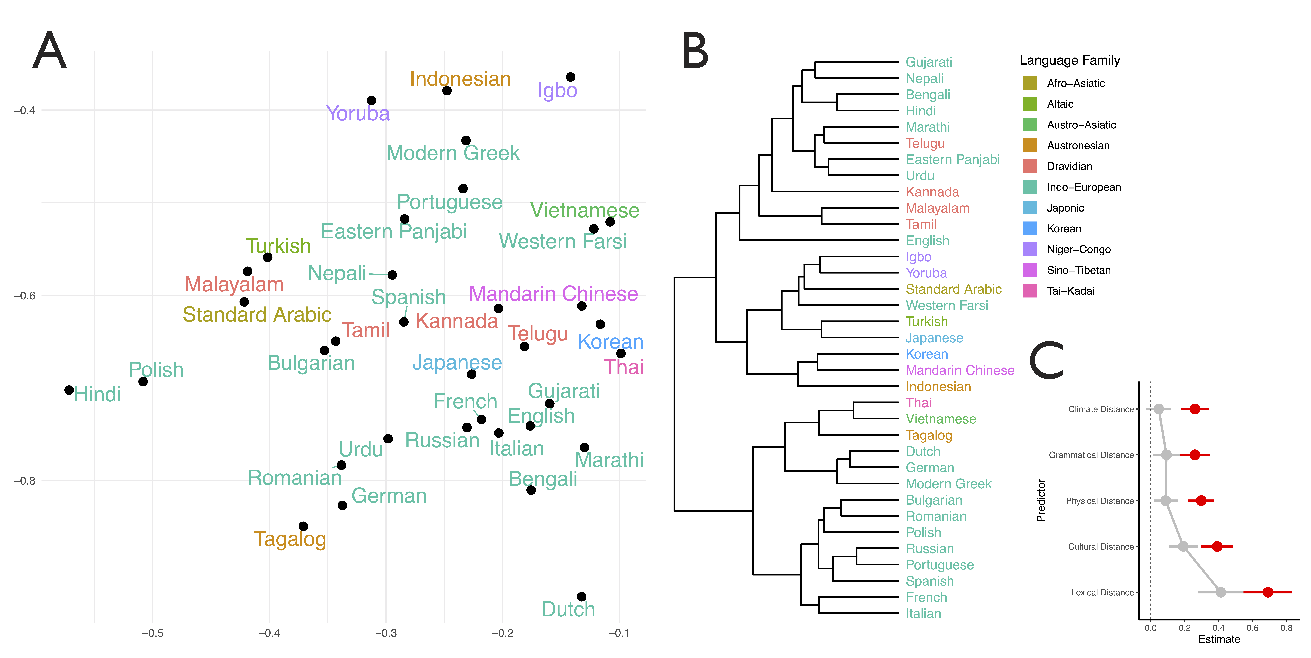
\includegraphics[width=16.7cm]{figs/fig2.pdf}
\caption{{\textbf A.} Two-dimensional projection of language centroids calculated from  document embeddings of the Second Language TOEFL Corpus. Color corresponds to language family. {\textbf B.} Hierarchical clustering of languages based on pairwise language distances of language centroids.; {\textbf C.} Standardized linear estimates of semantic distance predictors. Ranges are 95\% confidence intervals. Red points indicate estimates from single-predictor model; grey points indicate estimates from additive linear model with all five predictors included.}.
\label{fig:fig2} 
\end{figure*}



%4. Local similarity / global distance
\section*{Local similarity and global variability in semantic space} %[XXXXAdd discussion of Malt's conservation hypothesis!]
These analyses and theory motivate us to examine how languages vary in their structure at the ``system'' level across semantic domains. Across the semantic system, word meanings may differ in terms of their {\it local} semantic relations within a semantic domain -- e.g., the relative similarity of meanings associated with ``earth'' and ``sun'' (Fig.\ 3). Alternatively, meanings may differ in terms of their {\it global} semantic relationships across semantic domains -- e.g. the relative similarity of the ``astronomy'' cluster of meanings (``earth,'' ``sun,'' etc.) to the ``religion'' cluster (``spirit,'' ``hell,'' etc.; Figs. S11-S13). Finally, meanings may differ evenly across the system. 

Following Rosch, Mervis, and others \cite{rosch1975family}, we anticipated that locally clustered meanings would remain largely conserved across languages. They articulate how ```feathers', `wings', and `beaks''' frequently occur together' as constrained by shared experience with chickens in the world \cite{rosch1975family}. Elsewhere Malt and colleagues demonstrate how ``perception of stimulus properties by individuals interacts with linguistic and cultural histories, but their interaction is constrained by structure in the stimulus space'' \cite{Malt2003-vv,xu2020conceptual}. This perspective suggests that local clusters of meaning may be much more likely conserved across languages than farflung global associations that span the cultural system \cite[e.g.][]{lakoff2008women}. 

Supporting this expectation, we first found that word pairs from the same concreteness decile (``local'' relations) tended to cluster together and were more similar to each other across languages, relative to word pairs across concreteness deciles (``global'' relations; TOEFL:  $M$  $=$ 0.025, $SD$ $=$  0.005; $t$(594) $=$ 128.64; $p$ $<$ .0001; $d$ = 1.28 [1.15, 1.4];  $W$ = 177310, $p$ $<$ .0001; Wikipedia: $M$  $=$ 0.035, $SD$  $=$  0.015; $t$(594) $=$ 56.88; $p$ $<$ .0001;  $d$ = 0.27 [0.16, 0.39];  $W$ = 177272, $p$ $<$ .0001). Malt's work, however, casts doubt that the distinction between concrete and abstract words would account for the greatest cross-language variation. Her work reveals substantial cross-language variation in labels of the seemingly concrete domain of ``containers'' \cite{malt1999knowing, Malt2003-vv}, just as others have found substantial cross-language variation in body parts \cite{majid2015semantic, Levinson2006-bs}. This suggests that domain-clustered meanings may better account for variation in cross-linguistic semantic structure than the distinction between concrete and abstract concepts. 

To directly measure local-global semantic relations, which are not exclusively organized by concreteness, we clustered words according to their position within semantic space, and examined the relationship between words within and between clusters across languages (see Methods for detail; Fig. S14). Critically, we found that local semantic clusters were much more correlated across languages, relative to global semantic structure, and demonstrated stronger differences than between concreteness deciles in both the TOEFL ($M$  $=$ 0.058, $SD$ $=$  0.008;  $t$(594) = 185.97; $p$ $<$ .0001; $d$ = 2.84 [2.68, 3]; $W$ = 177310, $p$ $<$ .0001) and Wikipedia datasets ($M$  $=$ 0.038, $SD$  $=$  0.024; $t$(594) = 38.27; $p$ $<$ .0001;  $d$ = 0.31 [0.19, 0.42]; $W$ = 174402, $p$ $<$ .0001;  Figs.\ 4a-5; Figs.\ S15-S16). This effect was not related to the grammatical similarity of the languages (Fig. S4B, Fig. S17), showing remarkable consistency across languages (Figs. S18-S20). Further, the effect grew substantially larger as the number of semantic clusters increased (Fig. 3B, Fig. S21). 

% FIG 3
\begin{figure*}[t!]
\centering
\includegraphics[width=16cm]{figs/fig3.pdf}
\caption{{\textbf A.} Schematic representation of local and global distances in word embedding models. The figure shows three ``clusters'' of meanings and the relationships between them. Local relationships are within-cluster distances; global relationships are between-cluster distances. Some clusters are closer globally (e.g., $C_{music}$ and $C_{religion}$) than others (e.g., $C_{music}$ and $C_{war}$). {\textbf B.} Schema of the structure of cross-linguistic variability in local and global semantic structure. Each shading corresponds to a language. Languages tend to have overlapping clusters--to share local similarity--but vary in their global relations (e.g.  $C_{1}$ and $C_{2}$ are globally close in Language A, but not in Language B). {\textbf C.} Cross-linguistic word distance correlations for word groups in 10 semantic clusters based on words embeddings obtained from Second-Language TOEFL Corpus (top) and Multilingual Wikipedia Corpus (bottom). Red points indicate mean local correlation for each cluster, and blue squares indicate global correlation for each cluster.  {\textbf D.} Cross-linguistic word distance correlations for local versus global semantic comparison as a function of the number of semantic clusters. Point ranges correspond to 95\% confidence intervals.}
\label{fig:localglobal} 
\end{figure*}





\section*{Implications of cross-linguistic semantic diversity}
We find that variability in the structure of semantic space across languages is characterized by a high degree of similarity within semantic domains, but significantly more difference in the relationships between those domains. We interpret cross-linguistic variability in relations between semantic domains as creating measurable differences in the cognitive availability of linkages like associations, analogies, and metaphors that connect those domains. People who ``think'' in Greek cognitively follow and produce distinct semantic associations in language from others who ``think'' in Arabic, Farsi, Igbo or Chinese. Our research also characterizes the existence and extent of ``semantic accents'' previously identified in bilingual speakers \cite{matsuki2021understanding, dong2005shared} on large scales across the world's languages. 

Variability in global semantics has dramatic implications for cross-cultural communication and collaboration. It suggests that faithful, word-by-word translations are not possible, not because the objects of reference are uncertain \cite{quine2013word}, but because associations, metaphors and stories interlink different domains of meanings in one language culture than another \cite{lakoff1987categories}. This means that communication between two people of different language backgrounds will necessarily lead to some loss and distortion of intended meaning.  Further, it points to the intriguing possibility that communication will be more faithful among speakers of semantically more aligned languages:  A native speaker of Turkish can more effectively communicate in a second language with a native speaker of a semantically similar language, like Japanese, compared to a dissimilar one, like Dutch. 

Our findings invite future research to examine the cognitive consequences of cross-linguistic differences in semantic relations for non-native speakers. Previous research suggests how speakers of different languages may perceive  \cite{winawer2007russian, boutonnet2015words}, remember \cite{loftus1974reconstruction, latourrette2020naming, frank2008number, majid2004can, levinson2003space, pavlenko2011thinking}, and learn \cite{lupyan2007language, zettersten2020finding} about the world in different ways. Our work suggests that these effects may extend to  tasks that require linking clusters of meanings.  Future research could directly detect local-global semantic accents behaviorally using a classic priming paradigm \cite{dong2005shared}, with native and non-native speakers producing different associates in proportion to the semantic alignment shown here. Our work further predicts differences between native and non-native speakers in language comprehension that transcend native familiarity \cite{hayakawa2018using, costa2014your, keysar2012foreign}. Global semantic relations deployed in analogies or metaphors should be more difficult to process in one's second language relative to one's native language if those parts of the language do not align. In contrast, language relying on local semantic relationships should be easier to process, regardless of language. This prediction could be tested using behavioral measures like reaction time or neural signals, like N400 \cite{kutas2011thirty}, where we expect processing difficulty in proportion to the semantic distances we measure in this study (i.e., a larger N400 effect for more semantically distant cross-language word pairs). 

Domains that lie close within a language as assessed by our models are associated with an increased likelihood that speakers with native fluency transition from one concept to another across the proximate domain boundary \cite{arora2015random}. Transitions occur through discursive pivots within conversations, expositions, and narratives. They also occur in comparisons, such as similes and metaphors. We leave to future work the task of documenting whether specific types of transition (e.g., narrative turns vs. metaphors) become differentially likely with embedded proximity or whether all become more likely at a roughly equal rate as they are environmentally primed, reinforced, and become cognitively available to language speakers. 

Our findings also have powerful practical implications for language learning -- they suggest that learning words in a new language is not just a process of learning word forms and their mappings to referents, but also the higher-order association between their meanings. Currently, second-language training begins with explicitly translated word associations, often clustered locally within domains of experience (e.g., words for objects found in a house), interleaved with grammatical patterns required to use those words correctly in sentences. Later, language learners are introduced to global associations between clusters of meaning implicitly through native language literature and traditional stories. When people from a language write about family, do they also tend to link it with concepts of immutable stones and mountains, health, tragedy, or (in)justice? Our findings suggest discrepancies between native and non-native speakers in both comprehension and production could be reduced by training on the semantic associations in one's second language. Moreover, they point to the importance of recognizing that to speak with native fluency within a language, one needs to ``think'' in that language, producing global associations familiar to that language culture. 

Understanding how languages semantically vary also provides a new justification for the importance of cultural difference. Our findings could allow teachers and translators to compensate for semantic surprise and smooth intercultural communication. Artists, scientists, and scholars could equally leverage them to elevate disconnection and produce surprise. Recent scholarship on research innovation demonstrates how expeditions of academic outsiders produce the most unexpected and impactful findings. Only outside their scholarly languages do `alien' researcher insights and tools have the potential to generate novel solutions to previously intractable problems \cite{shi2023surprising}. Collective cognitive diversity might emerge from collaboration among those with native languages containing divergent semantic structures \cite{freeman2014collaboration}. Not only creators, but anyone making complex decisions could benefit from targeted confusion, where thinking like a native is more liability than benefit. 

One open question from our findings is the source of the cross-linguistic semantic differences we observe. For example, why do English and Persian differ in their semantic structure? In principle, two broad causal forces could lead to cross-linguistic variability. The first is variation in experience with the world, either from different physical environments or associations emergent from cultural life \cite{dale2012understanding, lupyan2015role,lupyan2016there,lupyan2010language}. For example, concepts of family and food might more closely associate for users of a language as a function of environmental capacity, resource abundance, and the ongoing tradition of family gathering to produce and consume food together. Other differences in experience follow from technological configurations and complexity, which also shape associations represented in language.

The second potential causal force is linguistic associations that violate experience. Consider homonymy, where two words with divergent meanings sound similar, or polysemy, where the same word holds different or divergent meanings. Homonymy and polysemy may arise through the merger of distinct language populations, or those previously separated where the dialects underwent functional evolution before re-merging. These historical `accidents' become apparent in the frequency of uncertain or competing etymologies, where word cognates and roots exist in multiple parent languages (e.g., Latin, Greek, and Saxon for English). Despite their `accidental' character, when similar or identical words link divergent meanings, they indirectly hyperlink other concepts and domains related to those linked \cite{aceves2021human}. This path-dependent process may channel progressively stronger semantic associations in language, inspiring material proximities that reinforce the association. In this way, the two potential causal forces -- experience with the world and linguistic accidents -- are not mutually exclusive and may recursively influence one another over time. Once linguistic associations become available for language speakers, however, they likely become reinforced through linguistic experience \cite{greenwald2017ai,lewis2020,  lewis2016length}. 

Using experimentation to understand the ways in which causal forces interact to drive the semantic variability we observe is an important target for future work. Using an artificial language learning paradigm \cite{kirby2008cumulative}, one could create concepts that hyperlink multiple meanings (i.e., novel homonyms) or teach new knowledge that functionally links them (e.g., novel composite technologies or theories), then evaluate the degree to which each contributes to altering the perceived distance between meanings \cite{lupyan2007language}. One could further stage experiments that compare linguistic accidents with altered embodied experiences \cite{casasanto2011different}. Alternatively, analysts could take a historical observational approach and measure the influence of historical accidents such as language mergers compared with changes in the emergence of new knowledge and technology, giving rise to functional shifts in the structure of meaning \cite[e.g.][]{pagel2007frequency}. 

Our analysis involves several limitations. First, we model language semantics in our analyses exclusively through word co-occurrence information captured through word embedding models. Prior work has demonstrated that estimates of meaning similarity derived from word embeddings are strongly correlated with explicit human judgments of word similarity \cite{hill2015simlex,pereira2016comparative}. Nevertheless, they do not perfectly correlate, suggesting that our method may not fully capture variability in cross-linguistic semantics. Contextual embeddings from the transformer models underlying modern chatbots \cite{vaswani2017attention, devlin2018bert, radford2018improving}, provide greater resolution by capturing the semantics of words in context, but they require more language data than the modest corpora available to us. Second, our corpora -- native language expository articles from Wikipedia and second language TOEFL essays -- reveal that there is cross-linguistic variability in connotative semantic associations, but we do not have comparable samples of fiction, poetry, conversation, or informal text to directly test this hypothesis. Finally, our data are correlational: behavioral experiments are needed to definitively establish the causal role of semantic space on the cognitive accessibility of semantic associations. % (the alternative hypothesis is that there's a third variable -- ''culture'')

Understanding how languages differ in their semantics has the potential to facilitate better cross-cultural communication, and provide a new justification of the importance of cultural difference.  Our work is the first to describe the general principles governing this variability and characterize these differences across semantic space.

%Discussion possibilities:
%(1) Understanding the precise nature and degree of cross-linguistic semantic variability is important because it holds cognitive implications for our ability to learn and switch between languages, just as it pinpoints the pitfalls and potential of intercultural communication around the world \cite{marti2023latent}. %To the extent to which language meanings are widely conserved \cite{wierzbicka1996semantics,fodor1975language, youn2016universal}, the process of learning a language or translating a document is simply the process of mapping linguistic forms to the same units of meaning. 
 
%(2) Systematic variability would suggest that learning words in a new language is not just a process of learning word forms and their mappings to referents, but also the higher-order association between their meanings. More specifically, understanding where pairs of languages vary greatest in close versus distant meanings could facilitate strategic training that prepares language learners to interpret disorienting associations, analogies, or turns of conversation and exposition. This insight would also allow language speakers to anticipate and, where desirable, avoid disorienting surprises when addressing persons from distinctive language groups.

%(3) Measured misalignment would also enable targeted semantic training for students from one specific language background learning another. Communication between people from different language backgrounds could lead to predictable distortions of intended meaning. This would have implications for cross-cultural communication, implying less friction among speakers of languages with greater semantic alignment, and more confusion but greater novelty among speakers with less alignment. 


% FIG 4
\begin{figure*}[t!]
\centering
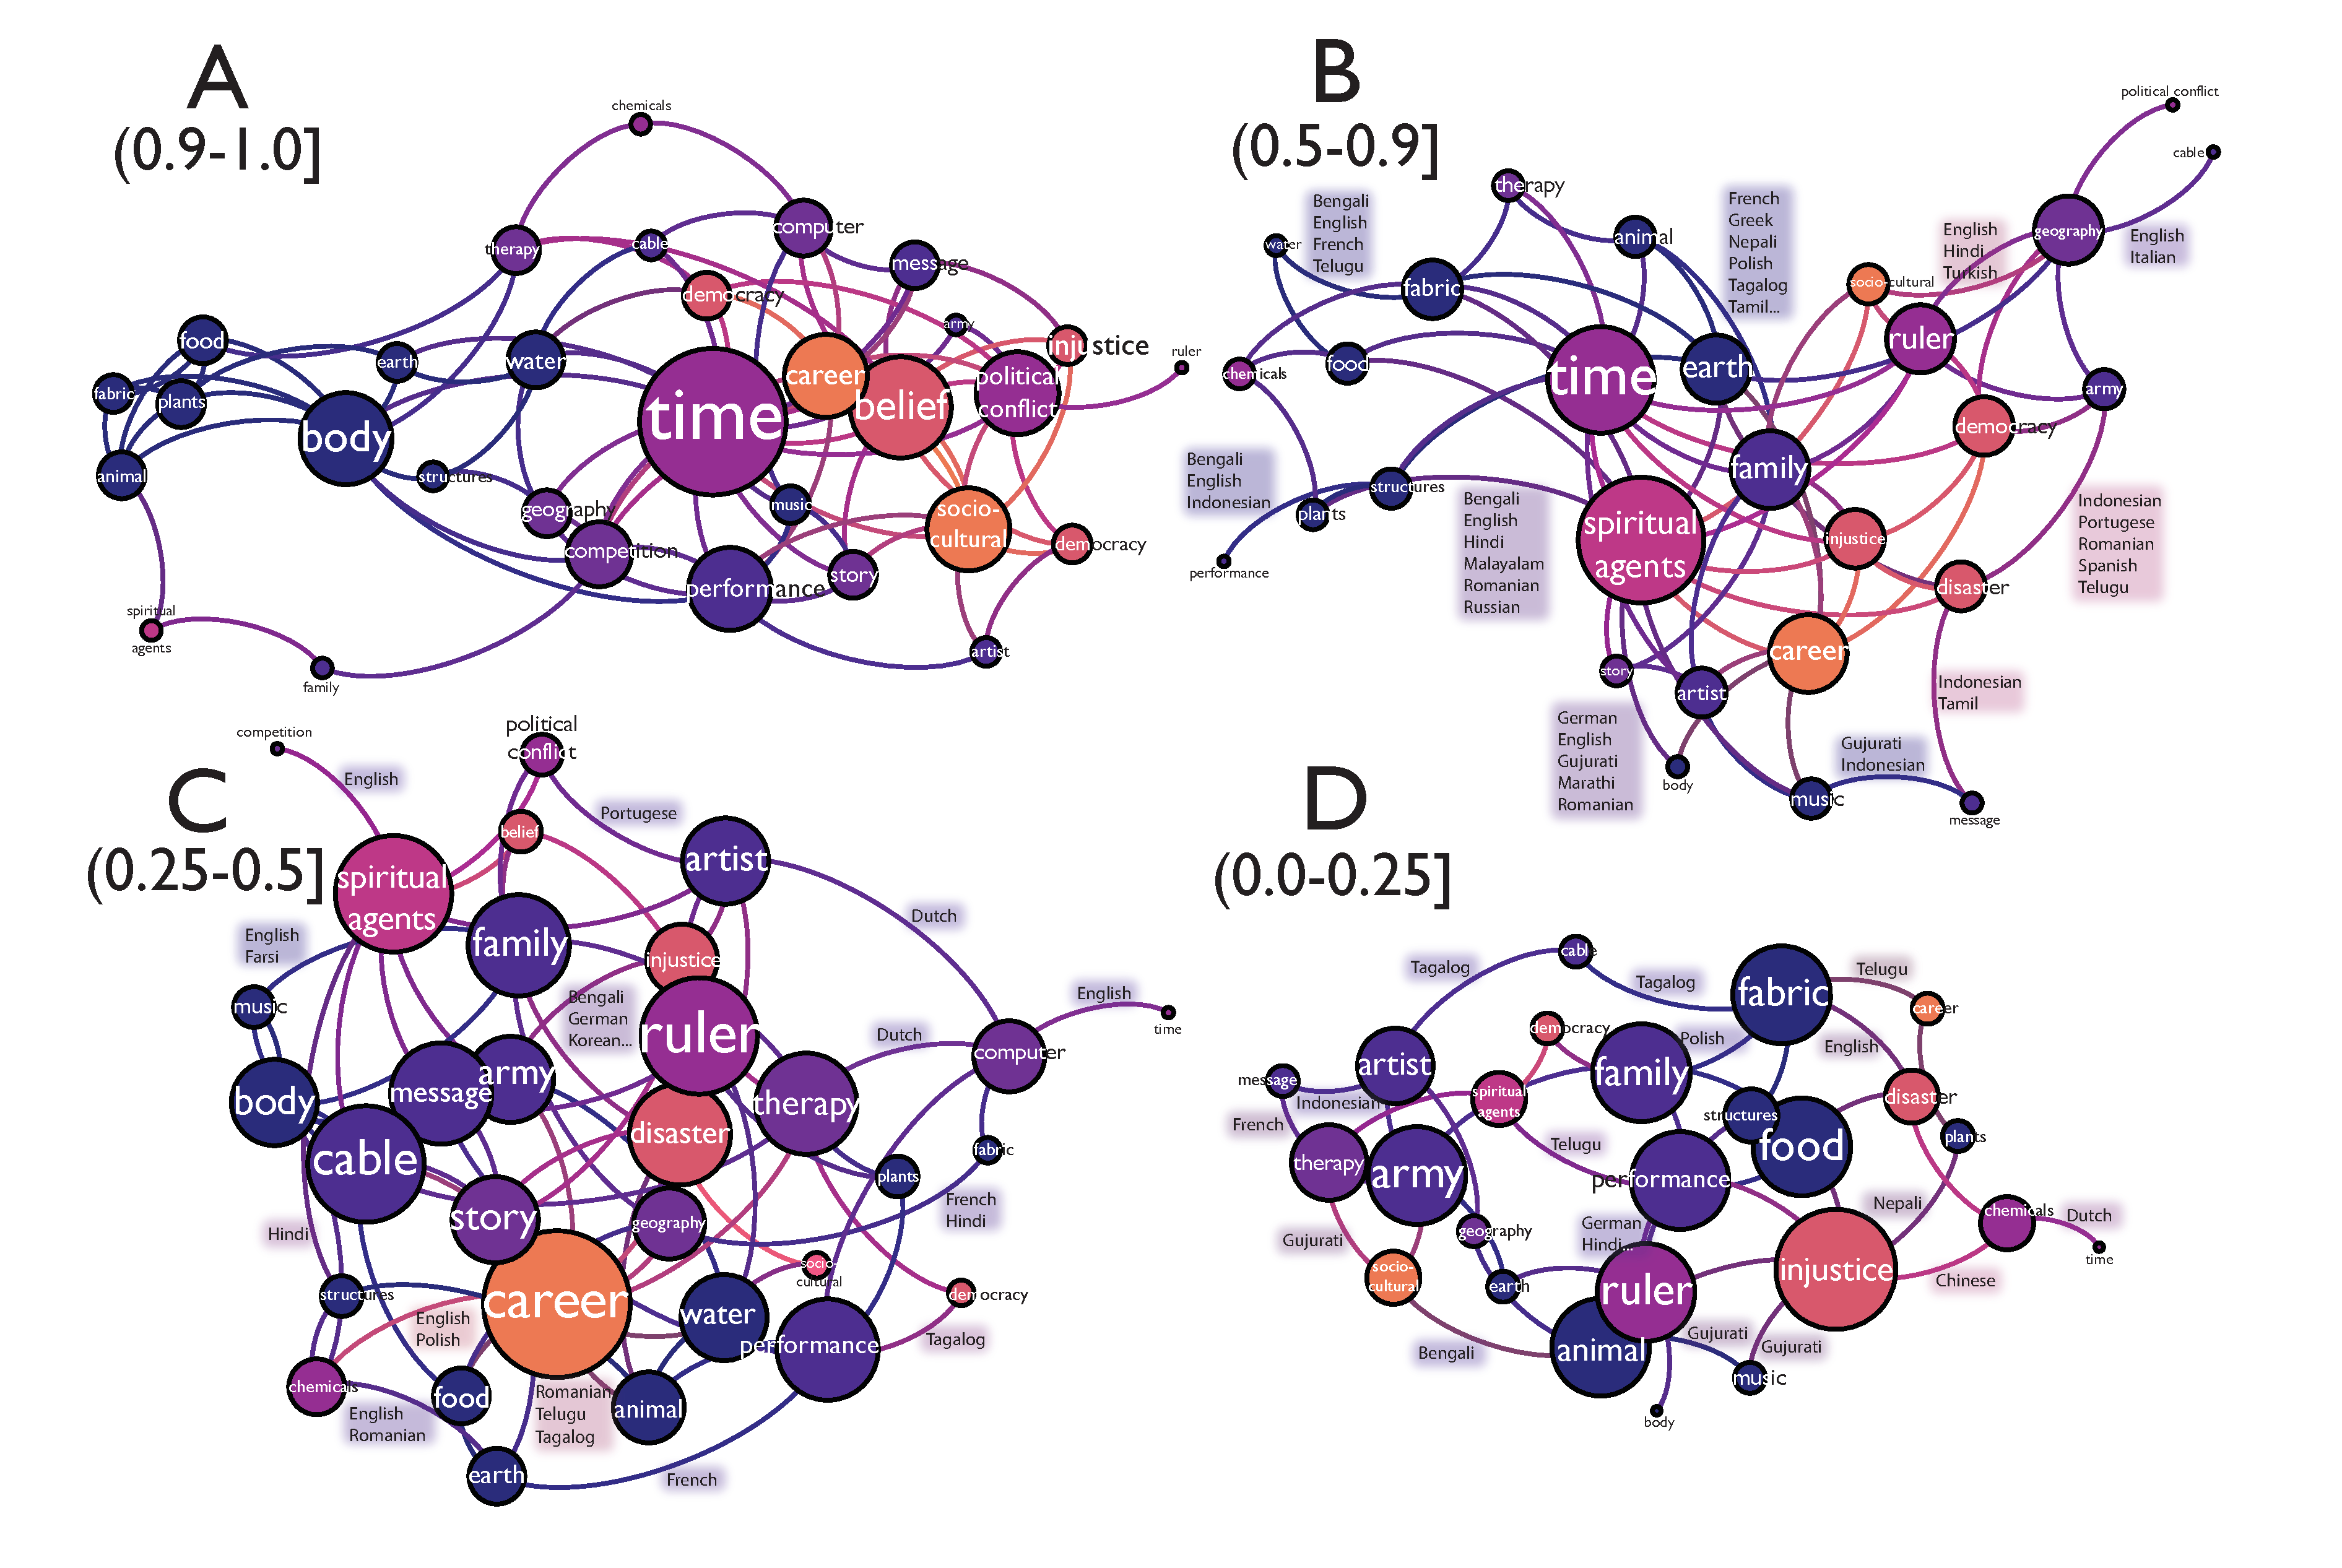
\includegraphics[width=16.7cm]{figs/fig4.pdf}
\caption{Semantic cluster graphs where links between clusters represent whether or not those clusters are within the top quartile of global semantic closeness for the proportion of languages that share both clusters specified above each graph. Links between clusters in Panel A are shared by almost all (0.9-1.0] languages in which the clusters manifest. Panels B-D represent global associations shared among fewer languages (0.5-0.9], (0.25-0.5], and (0.0-0.25]. These differences illustrate that despite stable, shared local semantic clusters across languages, global associations between those clusters vary dramatically. All graphs are rendered in 2D using force-directed algorithms that draw together the most connected clusters. See more details about data, cluster labels, and 2D layout in the Supplementary Information.}
\label{fig:fig4} 
\end{figure*}

\matmethods{Data and code are available through the GitHub repository associated with the project: \url{https://github.com/mllewis/SYSTEMSEM}.

\subsection*{Corpora and Models}
 The Second Language TOEFL corpus contained 38,500 short essays written in English by second-language learners of English. Each essay was written in response to one of 28 different essays prompts. The essays were written by equal number of participants from 35 different languages. Each essay was associated with a 1-5 score, implying an essay that ranged from poor to excellent. 

To evaluate whether each language was associated with a distinct semantic space, we trained a single \texttt{doc2vec} model \cite{le2014distributed} on this corpus with the output vector of 200 dimensions and a window size of 6.  We used the gensim implementation of the \texttt{doc2vec} model \cite{rehurek2011gensim}. For each target language, we then sampled 100 essays from each language and estimated the mean cosine distance within all essays in the target language and the mean cosine distance between essays in the target language and essays in other languages. We repeated this procedure 100 times for each language and estimated the mean within and between cosine distance in each language. To quantify the semantic distinctiveness of each language, we calculated the difference (and, alternatively, the ratio, see Fig. S2) of within to between essay distances. This value should exceed zero for differences (or one for ratios) if each language is associated with a distinct semantic space. We report both parametric ($t$-test) and non-parametric (Wilcoxon signed-rank test) analyses of the overall distinctiveness of essays by language, and within-language comparisons of distinctiveness for low versus high scoring essays. All tests are two-tailed.


All remaining analyses were performed on models trained on each language of the 35 languages separately.  Multilingual Wikipedia models were trained on corpora of Wikipedia articles in each of the target native languages using the \texttt{word2vec} skip-gram algorithm with default parameters \cite{bojanowski2016enriching}. The Second Language TOEFL models were trained on 35 corpora separated by the native language of the essay writer using the same training parameters as above. 



\subsection*{Word level analyses}

The conceptual concreteness of a word was estimated using previously-collected human judgments \cite{brysbaert2014concreteness}. Participants were presented with a single English word, and asked to rate the conceptual concreteness of its meaning on a 5-pt Likert scale, ranging from abstract to concrete.  The notions of concreteness and abstractness were defined for participants as follows: ``Some words refer to things or actions in reality, which you can experience directly through one of the five senses. We call these words concrete words. Other words refer to meanings that cannot be experienced directly but which we know because the meanings can be defined by other words. These are abstract words.'' Judgments were collected for a sample of 39,954 words.

For analyses using the Multilingual Wikipedia Corpus, we translated all words in the concreteness dataset into each of the target 35 languages using the Google Translate API. We selected the set of words that had translations for at least 30 of the languages, and then sampled 1,000 words from each of decile of concreteness (based on the human judgments described above). Of our target sample of words, 45\% of the translations existed in the embedding models across all languages.  For the Second Language TOEFL corpus, we selected all words that were present in the models of 5 or more languages ($N$ = 3,530 words). The words in this sample were roughly uniformly distributed across deciles.  Each word in our sample was rated for concreteness by at least 21 participants (TOEFL:  $M$  $=$ 54.9, $SD$ $=$  398; Wikipedia:  $M$  $=$ 37.5, $SD$ $=$ 236), and there was high agreement across participants in their rating of conceptual concreteness  (TOEFL: Mean $SD$ across words $=$  1.19; Wikipedia:  $SD$ $=$ 1.15).
 
 We compared word sets defined by different levels of concreteness to word sets defined by semantics. For both the Wikipedia and TOEFL models, we used k-means clustering \cite{hartigan1979algorithm} to cluster the words into 10 clusters each based on their semantics, through 50 iterations. To compare groupings by concreteness deciles and semantic clusters, we report in the main text the $\chi^2$ statistic of word counts in a $N$-cluster by concreteness decile matrix  (10 x 10; Fig.\ 1A). We also performed clustering for many other solutions, from 10 to 250 clusters, as shown in Fig.\ 3D, with greater differences between local and global correlations as cluster number grew. In Figure 3D, clusters were determined based on the model trained on English Wikipedia, using word loadings on the 300 Wikipedia embedding dimensions for all pairs of languages. We also created clusters based on the Wikipedia entries for every language in our sample ($N$ = 35).
 
 We next evaluated the semantic similarity of words across languages as a function of word concreteness (Fig.\ 1B). We calculated the pairwise distance (cosine; see methods below) between all words within each concreteness decile. We then calculated the correlation for these word distances for each language pairing ($N$ = 595). Finally, we averaged across language pairs to obtain an estimate of the mean cross-linguistic correlation in word distances across languages for each decile.  Correlation values are Pearson's $r$. 

To characterize cross-linguistic differences in local versus global similarity, we used the same set of words as above to compare  the pairwise cosine distances between words   in different concreteness deciles (``global'') to those in the same concreteness decile (``local'', described above). To measure  global alignment, we calculated the pairwise distance between words in different concreteness deciles, and then calculated the correlation for each language pairing and decile pairing (1-2, 1-3, 1-4, etc.). To measure local alignment, we calculated the pairwise distance between words in the same concreteness deciles, and then calculated the correlation for each language pairing and decile (1-1, 2-2, 3-3, etc.). We then compared the mean local correlation to the mean global correlation across language pairs ($N$ = 595). We report statistics for both parametric (paired $t$-test) and non-parametric (paired Wilcoxon signed-rank test) analyses. 

We conducted a parallel analysis using word sets defined by the semantic clusters (described above) rather than concreteness deciles, varying the number of clusters considered (10 - 250). In this analysis,       ``local'' refers to within-cluster distances and ``global'' refers to across-cluster distances. Means and standard deviations presented for these analyses correspond to the difference in correlation between local and global distances. Effect size measures are Cohen's $d$ and corresponding 95\% confidence interval. 

Finally, we replicated the cluster-based analysis using clusters determined by native language embeddings, rather than English-based clusters (Fig.\ S10). We performed pairwise comparisons of word distances within and across cluster boundaries, calculating this for TOEFL essays in both languages based on the cluster solution from each of the two languages, then averaging. For example, when comparing TOEFL essays from native Hindi and Mandarin speakers, we clustered words covering the Hindi and Chinese Wikipedia entries to capture how each language represents its knowledge base. Then we compared within Hindi-Wikipedia-clusters vs. between Hindi-Wikipedia-clusters for essays from native speakers of both languages; next we compared within Mandarin-Wikipedia-clusters vs. between Mandarin-Wikipedia clusters for the same essays; finally we averaged these differences. This manifests the same pattern of results as those derived from English clusters suggesting the insensitivity of our findings to distinct sources of semantic cluster structure. This, of course, reinforces our finding that local structure is much more similar across languages than global structure.

\subsection*{Semantic similarity in Swadesh words}
We used the Google Translate  API to translate the 22 words analyzed by Youn et al.\ (2016) \cite{swadesh1952lexico} (a subset of the Swadesh list) into each of our target 35 languages.  We included the variants analyzed by Youn et al.\ (e.g., ``day''/``daytime'', ``ash''/``ashes''), averaging across words referring to the same concept. We obtained translations for 96\% of the words across languages using this method. We then used these translations to obtain embedding coordinates for each concept in each language from the Wikipedia-trained embedding model \cite{bojanowski2016enriching}. In cases where translations were available for multiple word forms (e.g., ``day'' and ``daytime'') or the translations were composed of multiple forms, we averaged across vectors.  We  calculated the  pairwise distance (cosine) between each unique word pair (231 pairs)  in each language. Then, for each word, we estimated the correlation (Pearson's $r$) between these distances for  each language pair (595 language pairs). We estimated the physical distance between languages by obtaining the geographical coordinates of each language from Glottolog 2.7 \cite{HammarstroemEtAl2011Oslo} and calculating the geodesic distance (distance on an ellipsoid) between each language pair. Finally, we correlated the language-pairwise distance correlation coefficient with the language-pairwise physical distance metric and estimated $p$-values using the Quadratic Assignment Procedure (QAP) \cite{snapackage}. The QAP procedure estimates $p$-values in a way that accounts for the non-independence of observations (see methods below).

 Climate similarity was based on climate data obtained from WorldClim \cite{fick2017worldclim} on the basis of geographical coordinates from Glottolog 2.7 \cite{HammarstroemEtAl2011Oslo}. For each language pair, we  measured the Euclidean distance between estimates of mean and variance in temperature and precipitation. Measures of linguistic distance were obtained from \cite{dediu2018trees}. Grammatical distance between languages is based on similarity of 130 typological features for each language coded from the WALS database \cite{wals2013}.  Lexical similarity is based on the Levenshtein edit distance between the phonological forms of a standard set of 40 words in each language \cite{wichmann_asjp_2013} (ASJP16). Finally, cultural similarity is based on data from D-place, an ethnographic atlas of cultural traits \cite{kirby2016d,thompson2020cultural}. The cultural distance measure presented in Fig.\ 2c is an aggregate measure of cultural traits from 10 domains (``agriculture and vegetation,'' ``actions and technology, ``emotions and values,'' ``kinship,'' ``law,'' ``possession,'' ``religion and belief,'' ``social and political relations,'' ``the house,'' and ``the physical world.''). See Figure S10b for by-domain analyses. 

%cite this - https://journals.sagepub.com/doi/pdf/10.1177/0142723719892794
\subsection*{Cosine distance as similarity metric}
Similarity and distance between words in an embedding space is typically assessed using ``cosine similarity,'' the cosine of the angle between two word vectors (``cosine distance'' is one minus the cosine between vectors). This is preferred to the Euclidean (straight-line) distance due to properties of high-dimensional spaces that violate intuitions formed in two or three dimensions \cite{kozlowski2019geometry}. For example, as the dimensionality of a hypersphere grows, its volume shrinks relative to its surface area as more of that volume resides near the surface. The surface area of a unit circle surpasses its volume in three dimensions, but as the hypersphere’s dimension approaches infinity, its volume approaches zero. %We normalize all word vectors \cite{levy2015improving},Levy, Goldberg, and Dagan 2015) such that they lie on the surface of a hypersphere of same dimensionality as the space.

A geometric interpretation may be preferable to a probability one like the Kulback-Leibler Divergence or Wasserstein Distance because the distance between two probability distributions assumes independence and equal weight between each dimension, which is not the case for neural models like \texttt{word2vec} that approximate factorization of a (very) large matrix, with a monotonically decreasing influence of each dimension in describing the overall variation of the matrix \cite{levy2014neural}. 

\subsection*{QAP non-independence}
Multiple regression quadratic assignment procedures (MR-QAP) tests are permutation tests for multiple linear regression model coefficients for data organized in square matrices of relatedness among $n$ objects \cite{dekker2007sensitivity}. This data structure has been most common in studies of social networks, where variables indicate a relation between $n$ actors, but are equally applicable here, where we explore a distance relationship between $n$ languages. In both network, and distance cases, the rows and columns are explicitly not independent of one another, and so assumptions of identically and independently distributed data, required for linear regression are misplaced. MR-QAP permutation tests allow us to demonstrate that the autocorrelation among language pairs does not influence the regressed association that we find--that the distances between clusters is significantly more variable than the distances within clusters (e.g., the alpha estimated in the regression of global distances on local distances is significantly greater than 0.) It is common to have coefficients that look highly significant under a classical null hypothesis test and that remain insignificant under MR-QAP because the QAP null hypothesis accounts for autocorrelation. 

}

\showmatmethods{} % Display the Materials and Methods section

\acknow{We would like to thank the National Science Foundation \#1520074 to the University of Chicago for partial funding for this project.}

\showacknow{} % Display the acknowledgments section

% Bibliography
\bibliography{L2ETS_bib_clean.bib}

\end{document}
